%!TEX program = xelatex
%!BIB program = bibtex

\documentclass[cn,black,12pt,normal]{elegantnote}
\usepackage{float}
\usepackage{hyperref}
\usepackage{amsmath}
\usepackage{amssymb}
\usepackage{pdfpages}


\lstset{%
basicstyle=\linespread{0.8}\tt,
frame=single, %把代码用带有阴影的框圈起来
breaklines=true, %对过长的代码自动换行
}

\newcommand{\setParDef}{\setlength {\parskip} {0pt} }
\newcommand{\upcite}[1]{\textsuperscript{\textsuperscript{\cite{#1}}}}

\title{面向对象程序设计 42042002 \\ 作业: Fraction }
\author{学号:1951510 \hspace{30pt} 姓名:姜文渊}
\institute{Tongji University}
%\version{0.01}
% \date{\zhtoday}
\date{2022 年 7 月 13 日}
\begin{document}
% \setParDef
\maketitle

测试截图放在 \lstinline{imgs} 目录中。

\section{功能概览}

本次作业中用C++语言完成了完成一个分数类( fraction )的构建。分数类支持如下功能:
\begin{enumerate}
    \item 取负运算(例:+2/3 -> -2/3,或者 -2/3 -> +2/3)
    \item 求倒数(例:2/3 -> 3/2)
    \item 约分(例:6/9 -> 2/3)
    \item 从double型构造分数(例:0.25 -> 1/4)
    \item 从字符串构造分数(例“1/4”-> 1/4)
    \item \textbf{高精度}算术运算(加、减、乘、除)
    \item 关系运算(>、<、>=、<=、==、!=)
    \item 分数转换为字符串,显示分数:当出现分母为1时,只输出分子;当分子分母相同时输出1;当分母是0时报告异常
\end{enumerate}
由于笔者实现的 fraction 类的底层是基于字符串的计算,故而可以支持高精度的计算(实际取决于机器的内存大小)。为了方便手动测试该 fraction 类,笔者同时实现了一个简单的 REPL (Read-Eval-Print Loop,“读取-求值-输出”循环),支持通过命令行的方式使用该类。该 REPL 支持如下指令:
\begin{enumerate}
    \item \lstinline{help} 显示帮助信息
    \item \lstinline{init} 清空所有变量,重置工作区
    \item \lstinline{li [var_name:str] [a/b]} 分数变量赋值
    \item \lstinline{lf [var_name:str] [f: double]} 将浮点数转化为靠近的分数
    \item \lstinline{show [var_name:str]} 显示变量的值
    \item \lstinline{list} 显示工作区所有变量的值
    \item \lstinline{reduce [var:str]} 将分数化为最简形式
    \item \lstinline{neg [var:str]} 取负数
    \item \lstinline{inv [var:str]} 取倒数
    \item \lstinline{add/sub/mul/div [t:str] [s1:str] [s2:str]} 四则运算,\lstinline{t = s1 op s2}
    \item \lstinline{eq/gt/lt/geq/leq/neq [s1:str] [s2:str]} 比较运算,\lstinline{s1 op s2}
\end{enumerate}

若要在二次开发中使用笔者的分数类,需要引入以下源文件:
\begin{enumerate}
    \item \lstinline{mynat.h}
    \item \lstinline{mynat.cpp}
    \item \lstinline{myint.h}
    \item \lstinline{myint.cpp}
    \item \lstinline{fraction.h}
    \item \lstinline{fraction.cpp}
\end{enumerate}
并在使用到分数类的源码文件中引入 \lstinline{#include"fraction.h"} ,然后即可使用 fraction 类。具体接口见 \lstinline{fraction.h} 。

\section{功能测试}

这些测试里没有对输出进行单独的测试,因为每种测试中都涉及到输出。

\subsection{分数的构造}

\paragraph{正整数} 测试用例 \lstinline{li a 8554334545345245254254125643}
\begin{figure}[H]
    \centering
    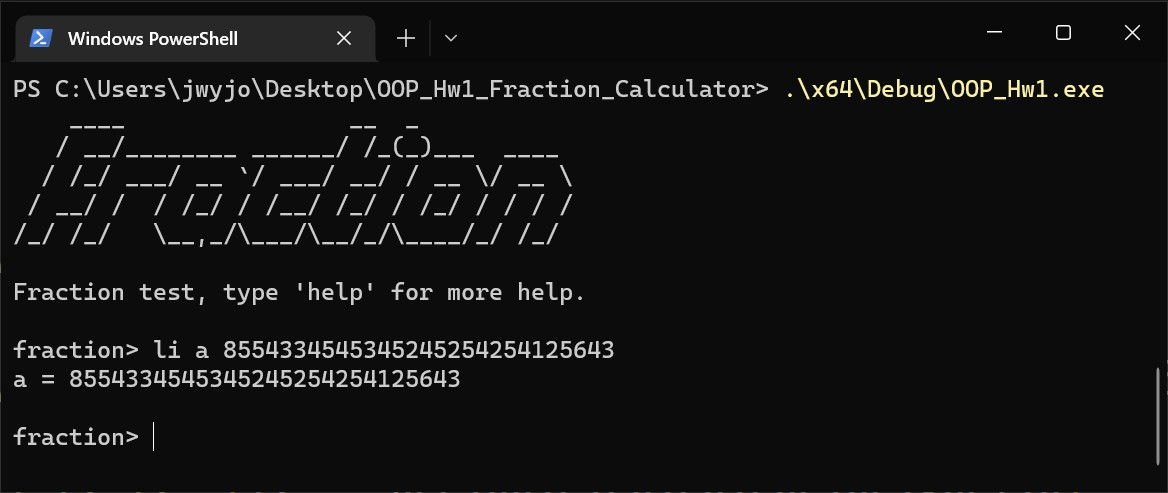
\includegraphics[width=.8\textwidth]{imgs/test_construct_positive_int.jpg}
    \caption{分数的构造-正整数测试结果(符合预期)}
\end{figure}

\paragraph{正分数} 测试用例 \lstinline{li a 85543351/8554334545345245254254125643}
\begin{figure}[H]
    \centering
    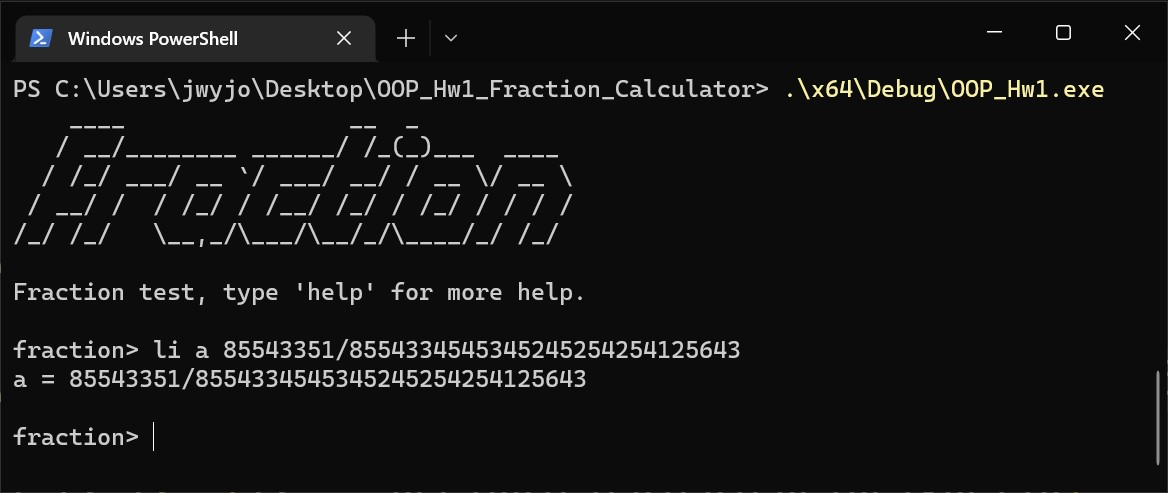
\includegraphics[width=.8\textwidth]{imgs/test_construct_positive_frac.jpg}
    \caption{分数的构造-正分数测试结果(符合预期)}
\end{figure}

\paragraph{负整数} 测试用例 \lstinline{li a -8554334545345245254254125643}
\begin{figure}[H]
    \centering
    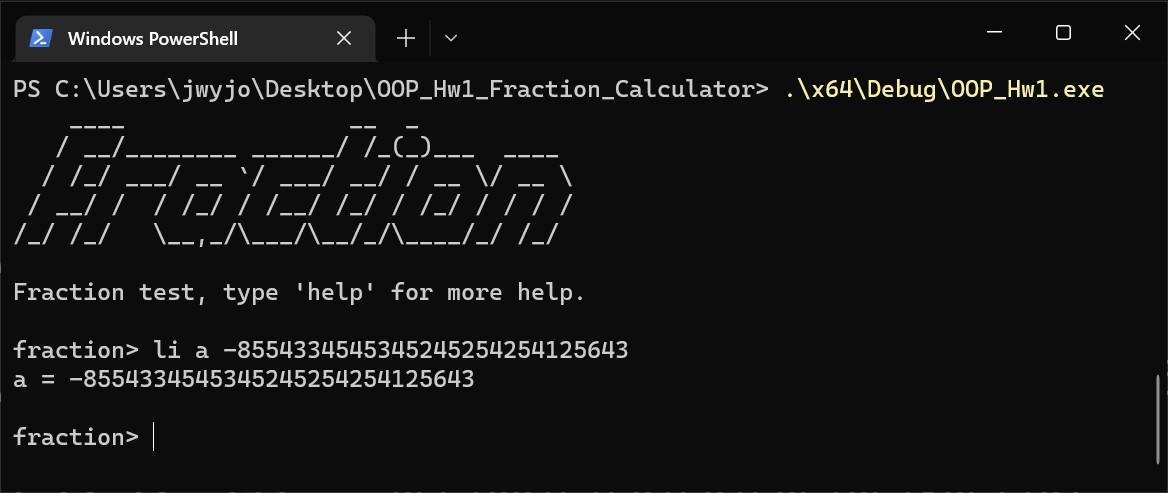
\includegraphics[width=.8\textwidth]{imgs/test_construct_negative_int.jpg}
    \caption{分数的构造-负整数测试结果(符合预期)}
\end{figure}

\paragraph{负分数} 测试用例 \lstinline{li a -85543351/8554334545345245254254125643}
\begin{figure}[H]
    \centering
    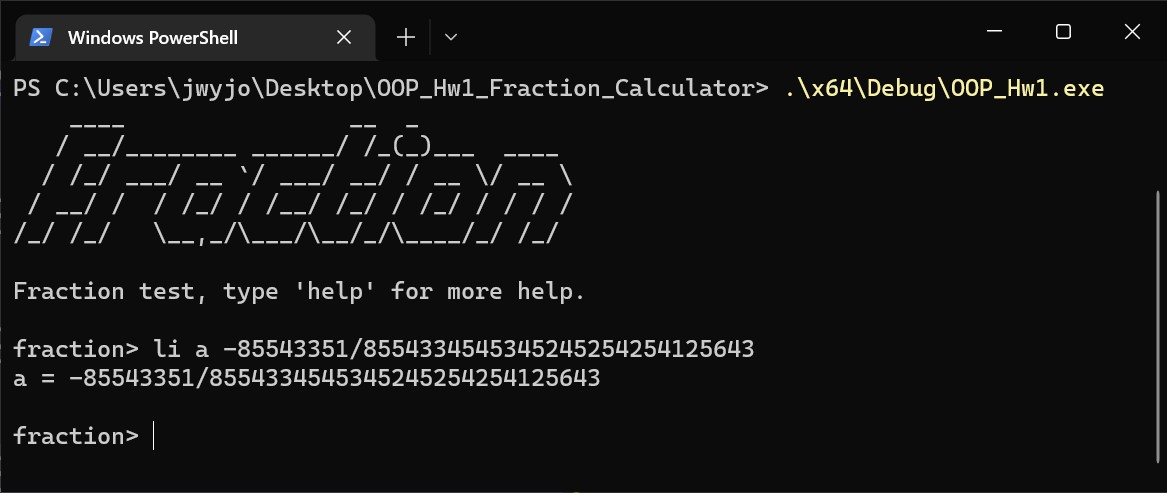
\includegraphics[width=.8\textwidth]{imgs/test_construct_negative_frac.jpg}
    \caption{分数的构造-负分数测试结果(符合预期)}
\end{figure}

\paragraph{零} 测试用例 \lstinline{li a 0}
\begin{figure}[H]
    \centering
    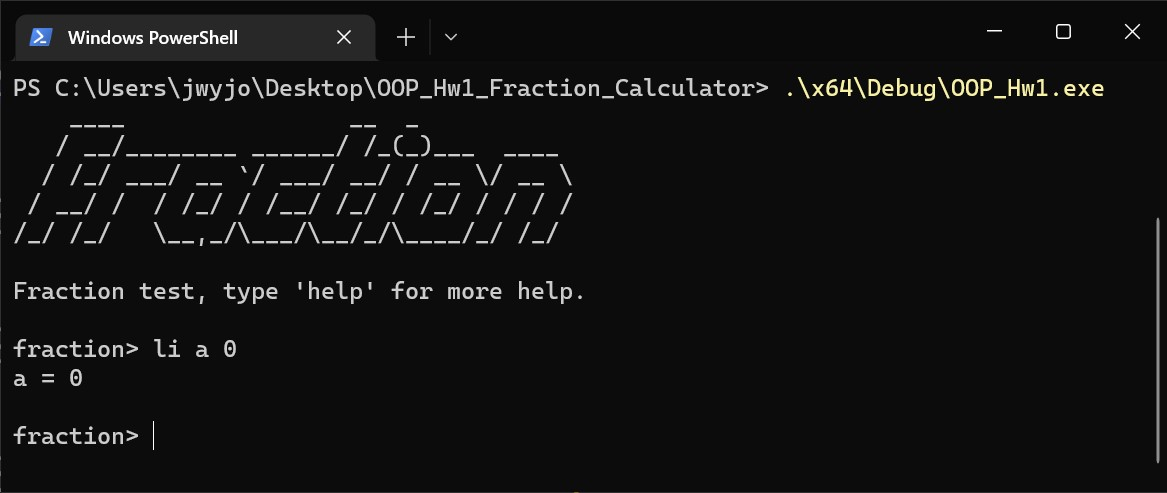
\includegraphics[width=.8\textwidth]{imgs/test_construct_zero.jpg}
    \caption{分数的构造-零的测试结果(符合预期)}
\end{figure}
\paragraph{正浮点数} 测试用例 \lstinline{lf a 0.85543345}
\begin{figure}[H]
    \centering
    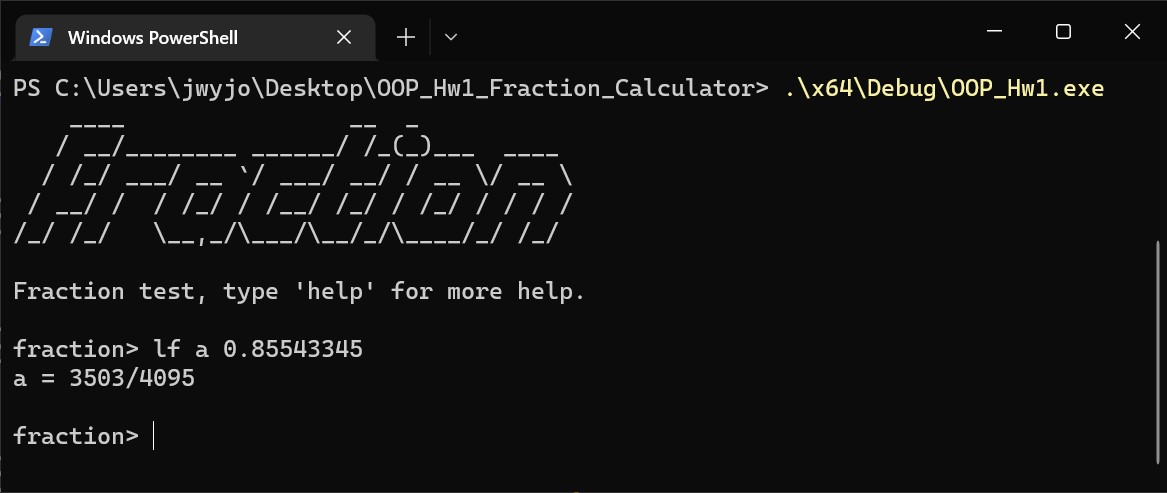
\includegraphics[width=.8\textwidth]{imgs/test_construct_positive_float.jpg}
    \caption{分数的构造-正浮点数测试结果(符合预期)}
\end{figure}

\paragraph{负浮点数} 测试用例 \lstinline{lf a -0.85543345}
\begin{figure}[H]
    \centering
    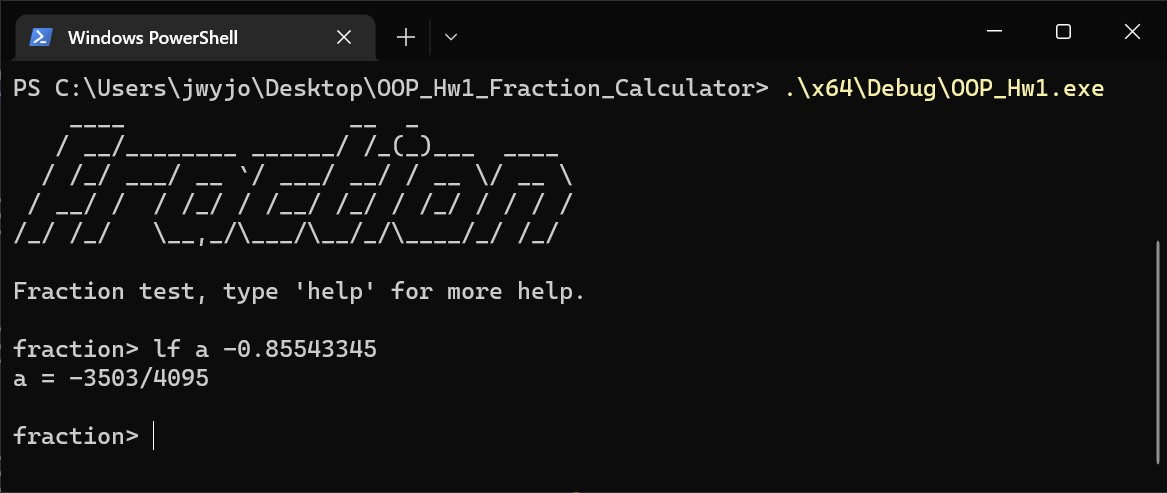
\includegraphics[width=.8\textwidth]{imgs/test_construct_negative_float.jpg}
    \caption{分数的构造-负浮点数测试结果(符合预期)}
\end{figure}

\subsection{分数的化简}

\paragraph{正分数} 测试用例 \lstinline{549755813888/1099511627776}
\begin{figure}[H]
    \centering
    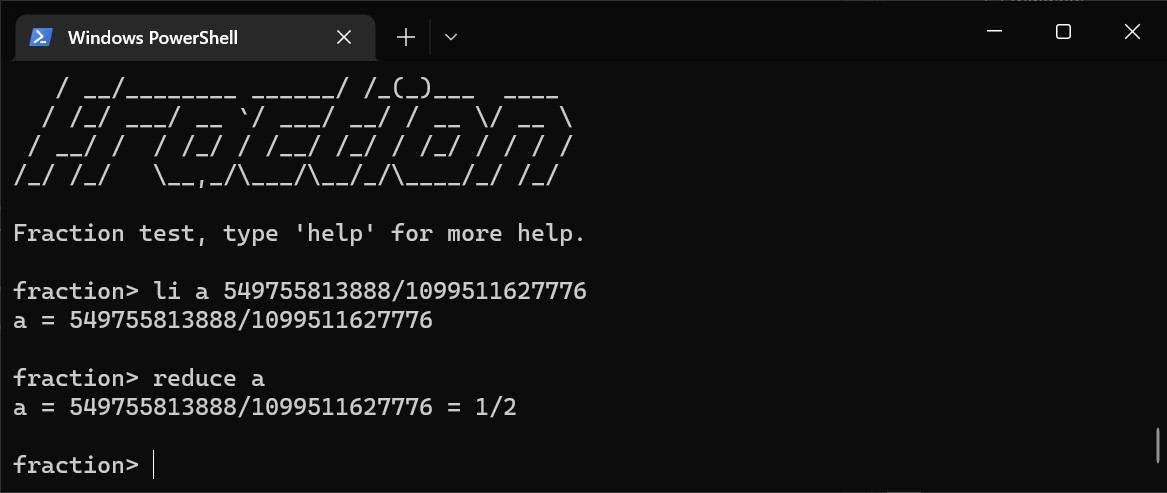
\includegraphics[width=.8\textwidth]{imgs/test_reduce_positive_frac.jpg}
    \caption{分数的化简-正分数测试结果(符合预期)}
\end{figure}

\paragraph{负分数} 测试用例 \lstinline{-549755813888/1099511627776}
\begin{figure}[H]
    \centering
    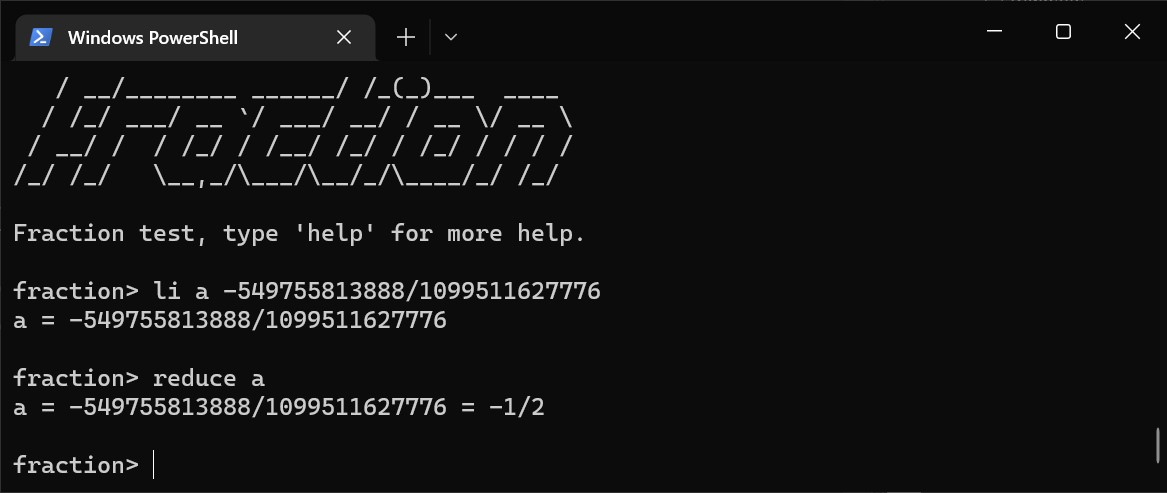
\includegraphics[width=.8\textwidth]{imgs/test_reduce_negative_frac.jpg}
    \caption{分数的化简-负分数测试结果(符合预期)}
\end{figure}

\paragraph{正整数} 测试用例 \lstinline{1099511627776/549755813888}
\begin{figure}[H]
    \centering
    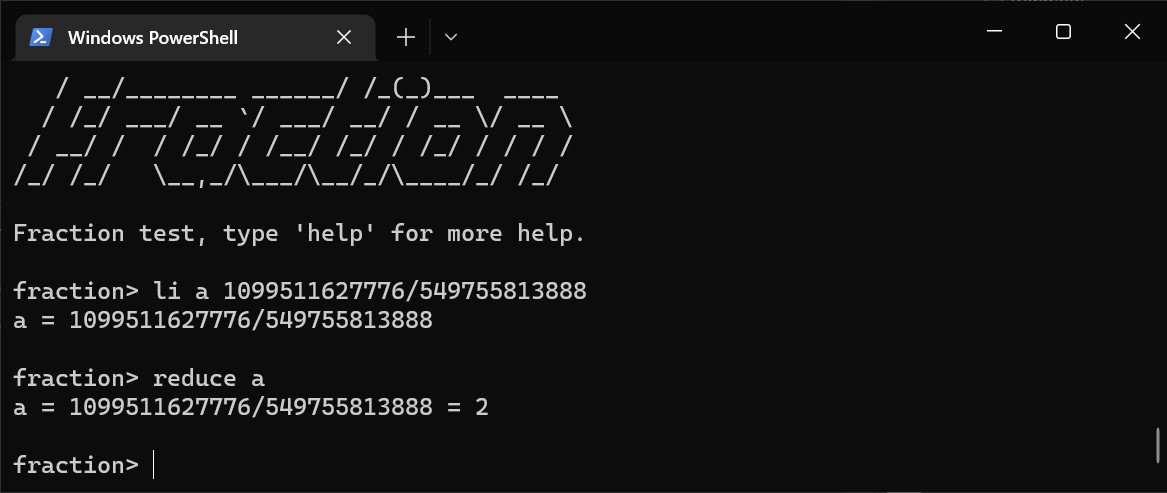
\includegraphics[width=.8\textwidth]{imgs/test_reduce_positive_int.jpg}
    \caption{分数的化简-正整数测试结果(符合预期)}
\end{figure}

\paragraph{负整数} 测试用例 \lstinline{-1099511627776/549755813888}
\begin{figure}[H]
    \centering
    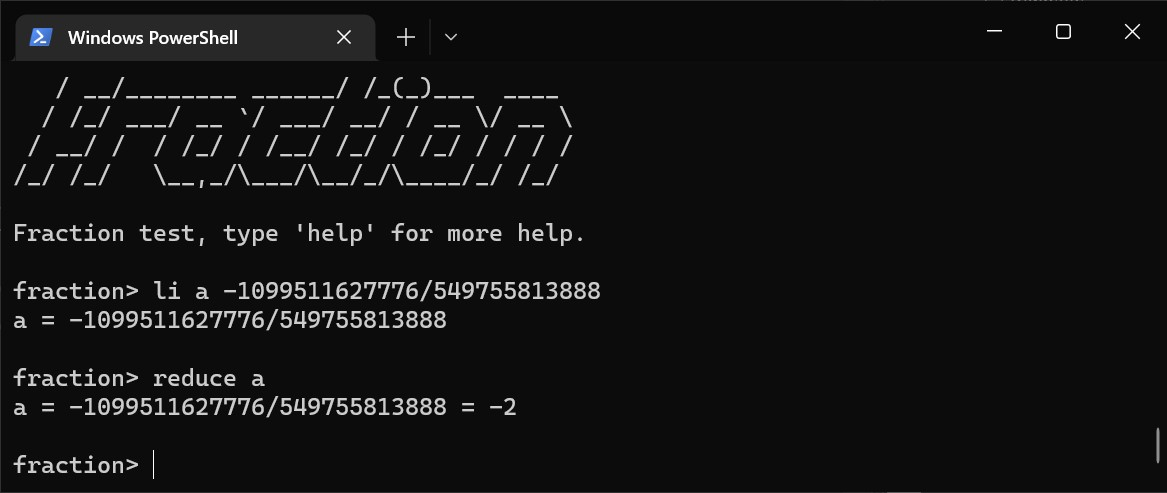
\includegraphics[width=.8\textwidth]{imgs/test_reduce_negative_int.jpg}
    \caption{分数的化简-负整数测试结果(符合预期)}
\end{figure}

\paragraph{零分母} 测试用例 \lstinline{1/0}
\begin{figure}[H]
    \centering
    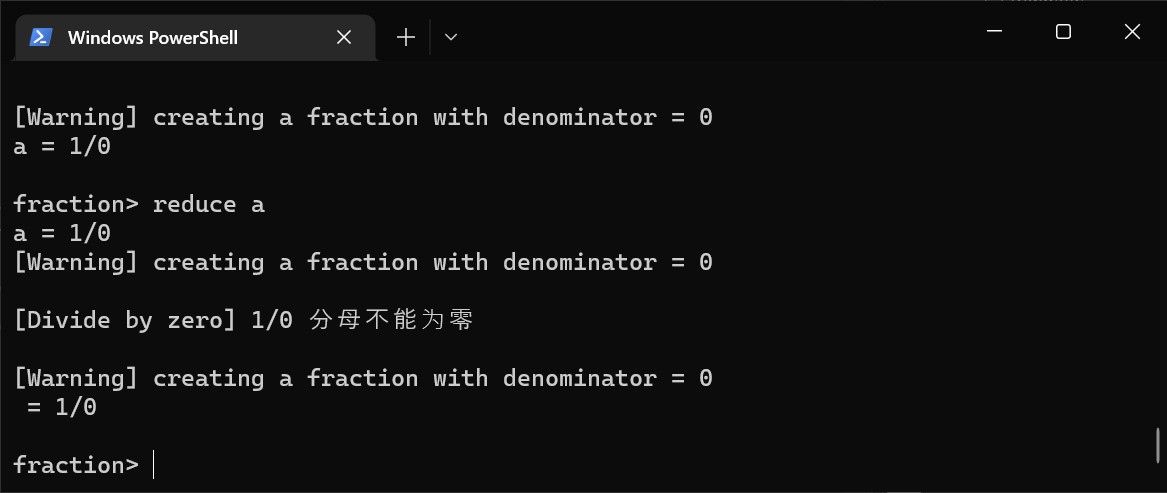
\includegraphics[width=.8\textwidth]{imgs/test_reduce_zero1.jpg}
    \caption{分数的化简-零分母测试结果(符合预期)}
\end{figure}

\paragraph{零分子} 测试用例 \lstinline{0/1099511627776}
\begin{figure}[H]
    \centering
    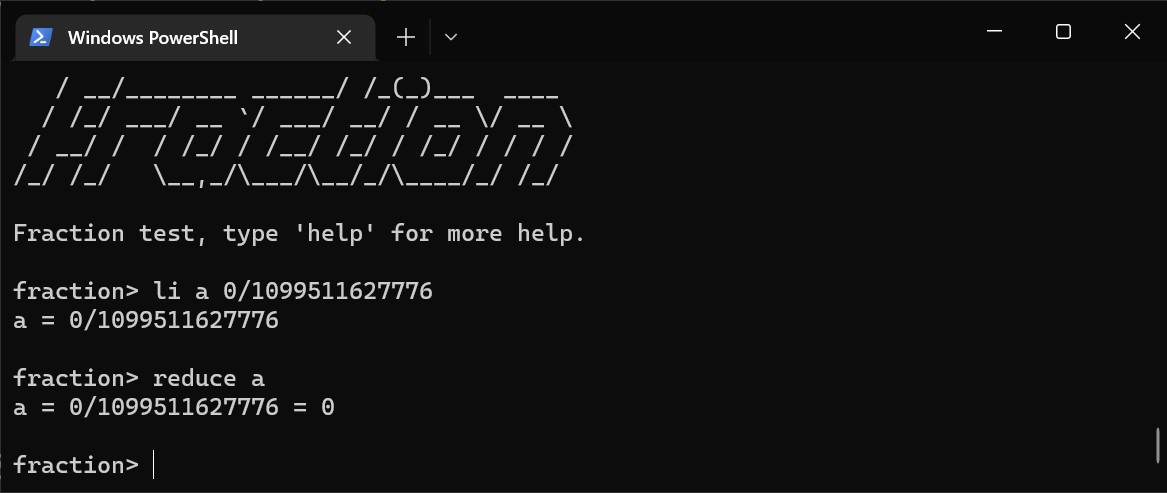
\includegraphics[width=.8\textwidth]{imgs/test_reduce_zero2.jpg}
    \caption{分数的化简-零分母测试结果(符合预期)}
\end{figure}

\subsection{取负数}

\paragraph{正数} 测试用例 \lstinline{549755813888/1099511627776}
\begin{figure}[H]
    \centering
    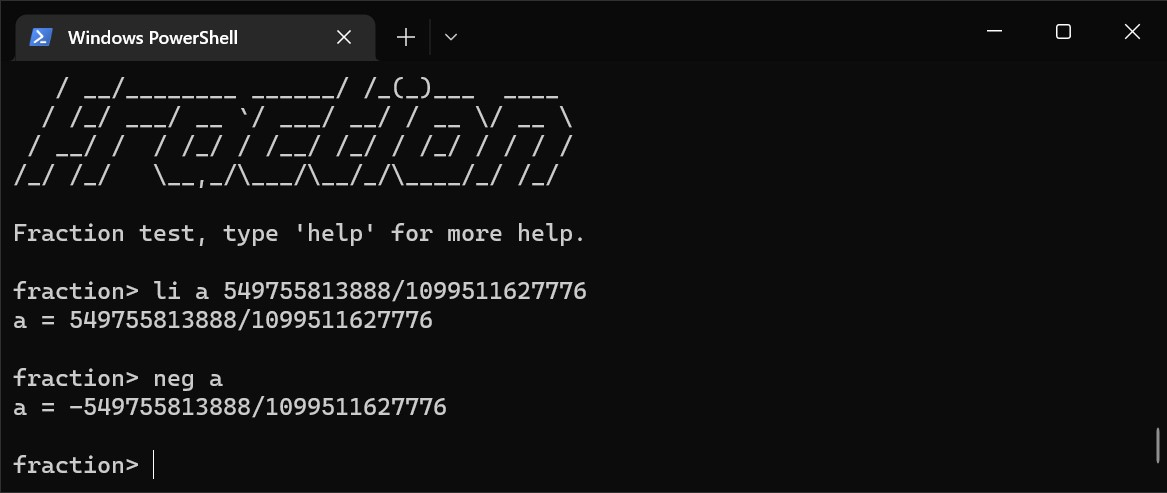
\includegraphics[width=.8\textwidth]{imgs/test_neg_positive_frac.jpg}
    \caption{取负数-正分数测试结果(符合预期)}
\end{figure}

\paragraph{负数} 测试用例 \lstinline{-549755813888/1099511627776}
\begin{figure}[H]
    \centering
    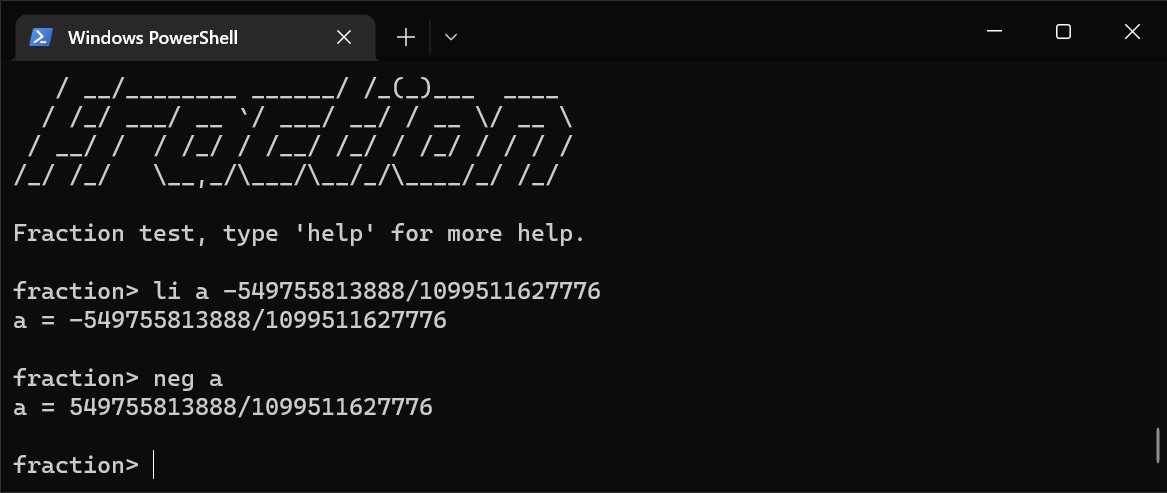
\includegraphics[width=.8\textwidth]{imgs/test_neg_negative_frac.jpg}
    \caption{取负数-负分数测试结果(符合预期)}
\end{figure}

\paragraph{零分母} 测试用例 \lstinline{1/0}
\begin{figure}[H]
    \centering
    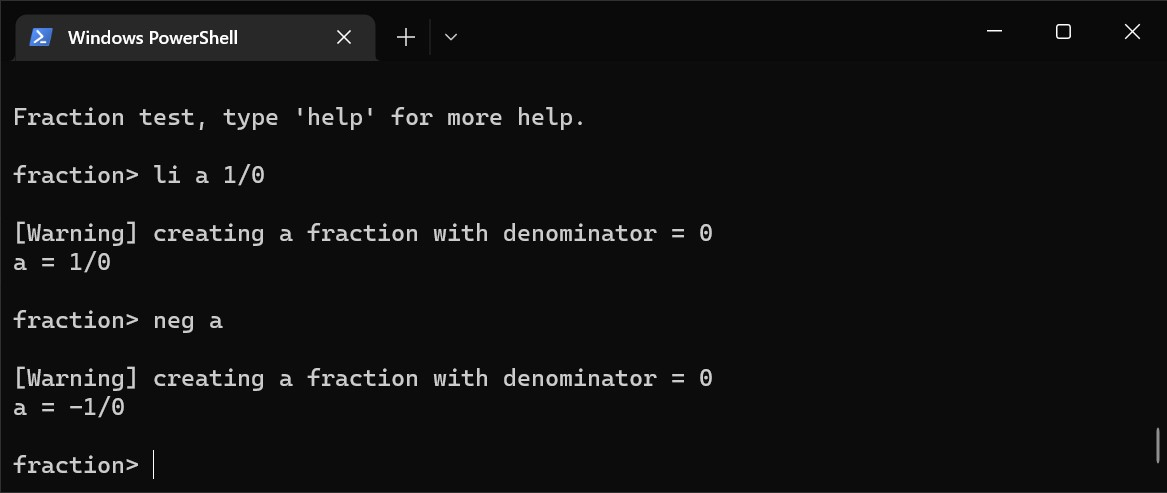
\includegraphics[width=.8\textwidth]{imgs/test_neg_zero1.jpg}
    \caption{取负数-零分母测试结果(符合预期)}
\end{figure}

\paragraph{零分子} 测试用例 \lstinline{0/1099511627776}
\begin{figure}[H]
    \centering
    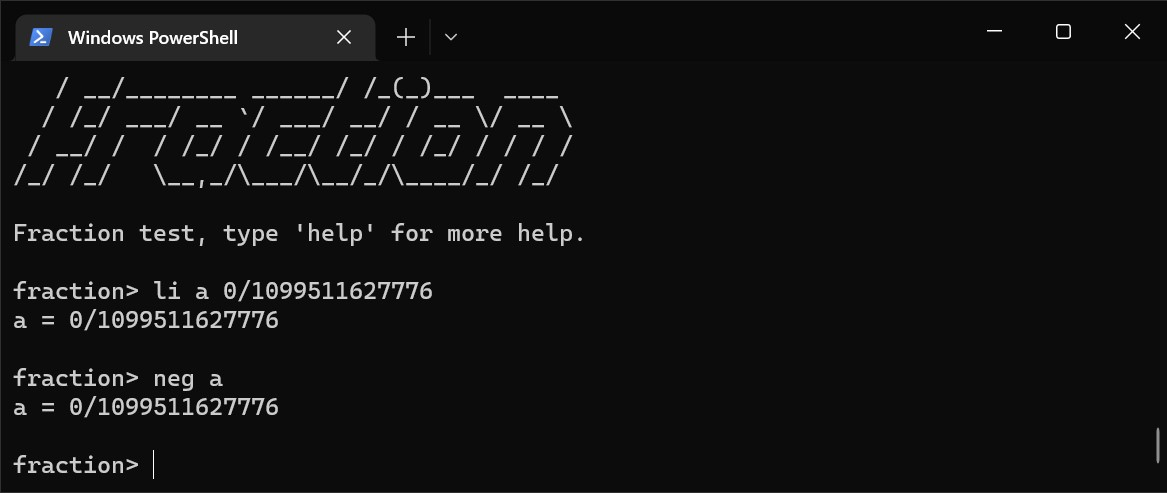
\includegraphics[width=.8\textwidth]{imgs/test_neg_zero2.jpg}
    \caption{取负数-零分母测试结果(符合预期)}
\end{figure}

\subsection{取倒数}

\paragraph{正数} 测试用例 \lstinline{549755813888/1099511627776}
\begin{figure}[H]
    \centering
    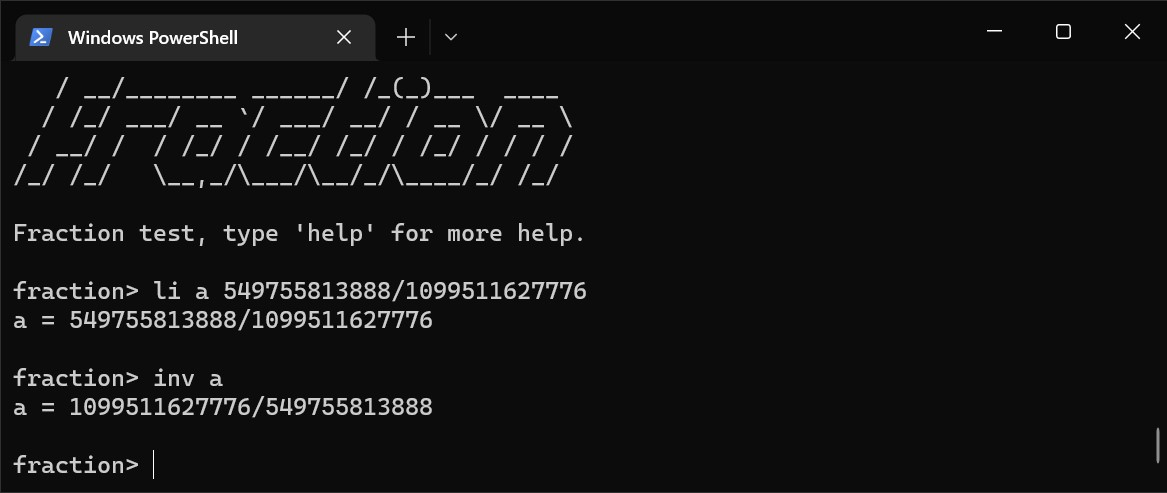
\includegraphics[width=.8\textwidth]{imgs/test_inv_positive_frac.jpg}
    \caption{取倒数-正分数测试结果(符合预期)}
\end{figure}

\paragraph{负数} 测试用例 \lstinline{-549755813888/1099511627776}
\begin{figure}[H]
    \centering
    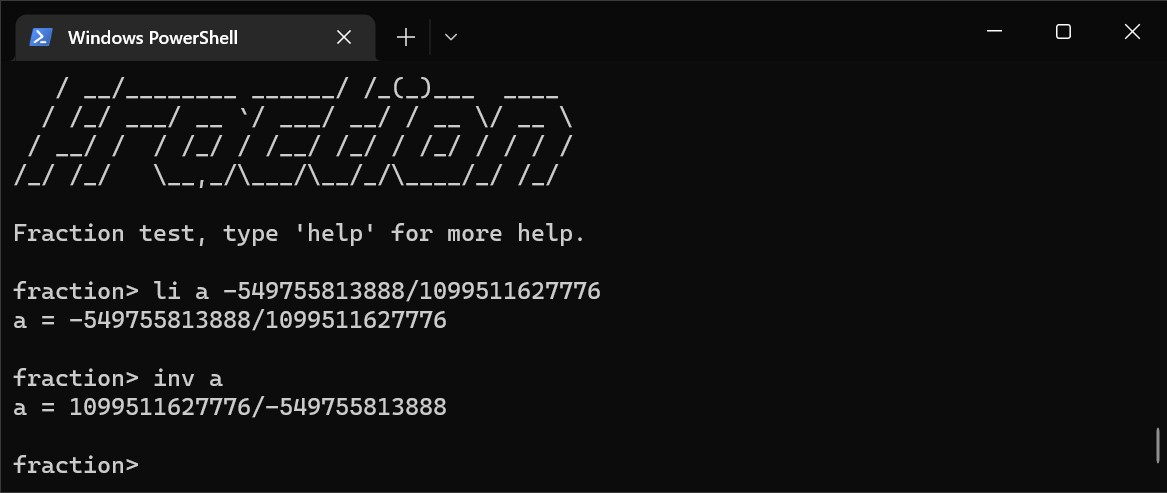
\includegraphics[width=.8\textwidth]{imgs/test_inv_negative_frac.jpg}
    \caption{取倒数-负分数测试结果(符合预期)}
\end{figure}

\paragraph{零分母} 测试用例 \lstinline{1/0}
\begin{figure}[H]
    \centering
    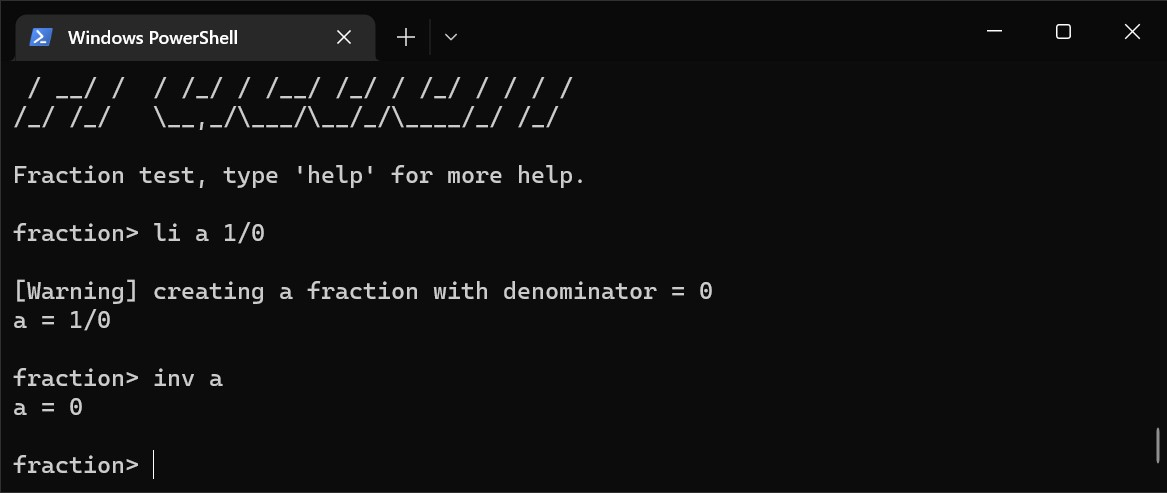
\includegraphics[width=.8\textwidth]{imgs/test_inv_zero1.jpg}
    \caption{取倒数-零分母测试结果(符合预期)}
\end{figure}

\paragraph{零分子} 测试用例 \lstinline{0/1099511627776}
\begin{figure}[H]
    \centering
    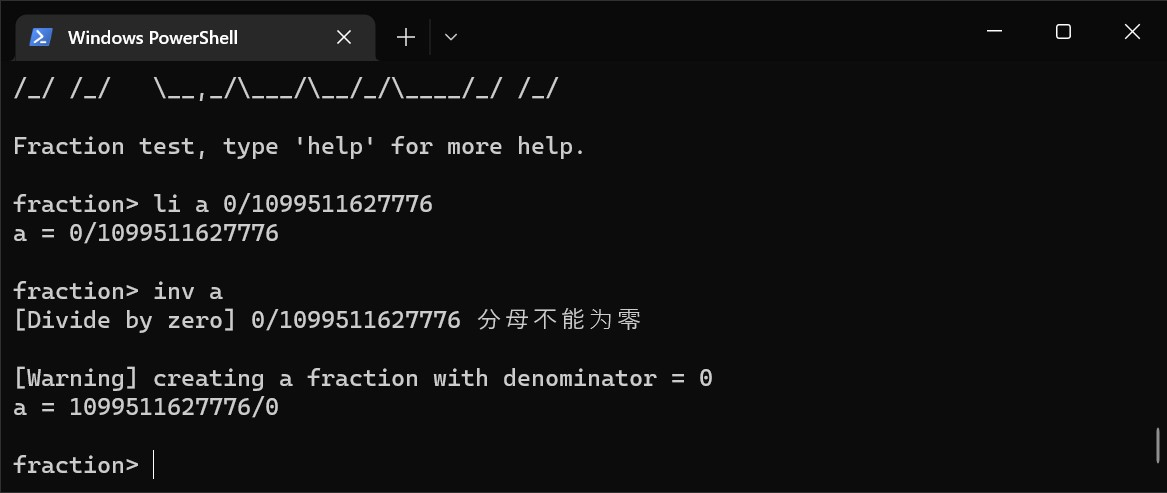
\includegraphics[width=.8\textwidth]{imgs/test_inv_zero2.jpg}
    \caption{取倒数-零分母测试结果(符合预期)}
\end{figure}

\subsection{四则运算}

\paragraph{加法} 测试用例 \lstinline{549755813888/1099511627776 + 1/-3}
\begin{figure}[H]
    \centering
    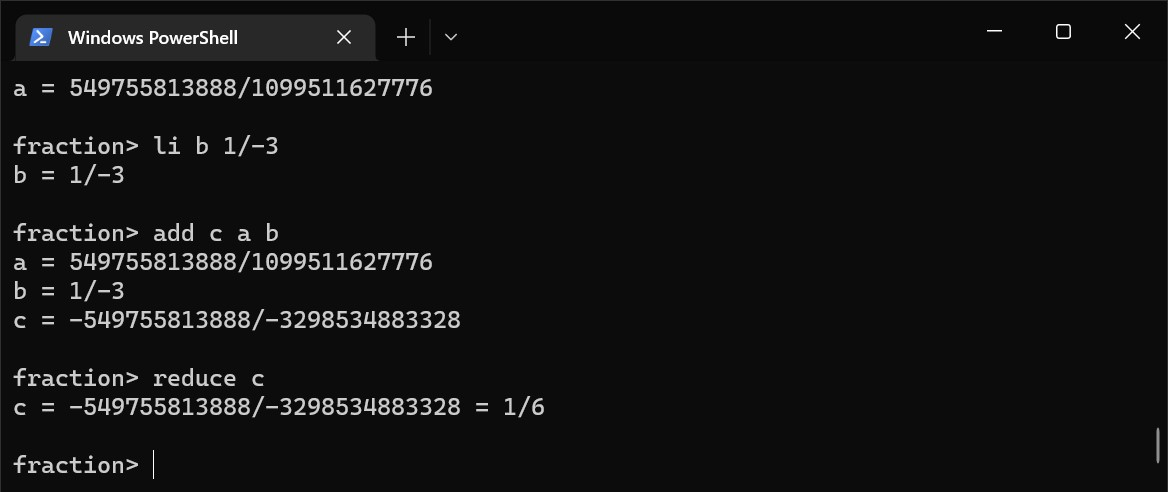
\includegraphics[width=.8\textwidth]{imgs/test_op_add.jpg}
    \caption{四则运算-加法测试结果(符合预期)}
\end{figure}

\paragraph{减法} 测试用例 \lstinline{549755813888/1099511627776 - 1/-3}
\begin{figure}[H]
    \centering
    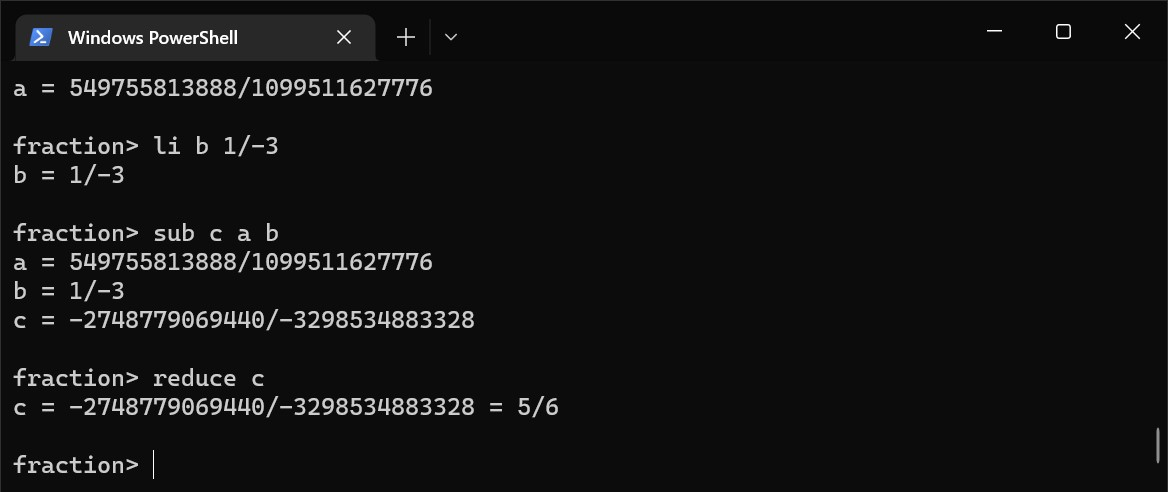
\includegraphics[width=.8\textwidth]{imgs/test_op_sub.jpg}
    \caption{四则运算-减法测试结果(符合预期)}
\end{figure}

\paragraph{乘法} 测试用例 \lstinline{549755813888/1099511627776 * 1/-3}
\begin{figure}[H]
    \centering
    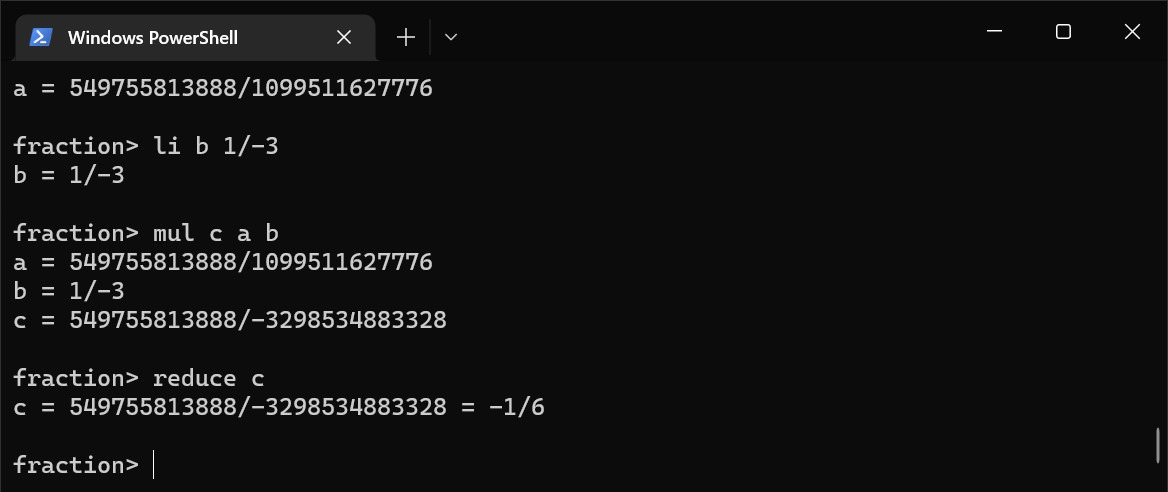
\includegraphics[width=.8\textwidth]{imgs/test_op_mul.jpg}
    \caption{四则运算-乘法测试结果(符合预期)}
\end{figure}

\paragraph{除法} 测试用例 \lstinline{549755813888/1099511627776 / 1/-3}
\begin{figure}[H]
    \centering
    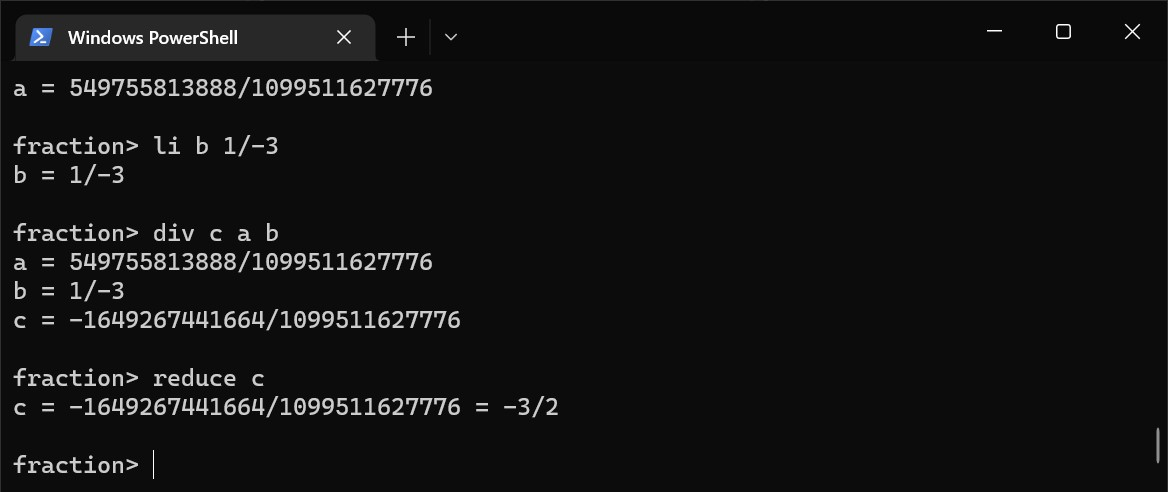
\includegraphics[width=.8\textwidth]{imgs/test_op_div.jpg}
    \caption{四则运算-除法测试结果(符合预期)}
\end{figure}

\subsection{比较运算}

\paragraph{大于} 测试用例 \lstinline{-549755813888/1099511627776 > 1/-3}
\begin{figure}[H]
    \centering
    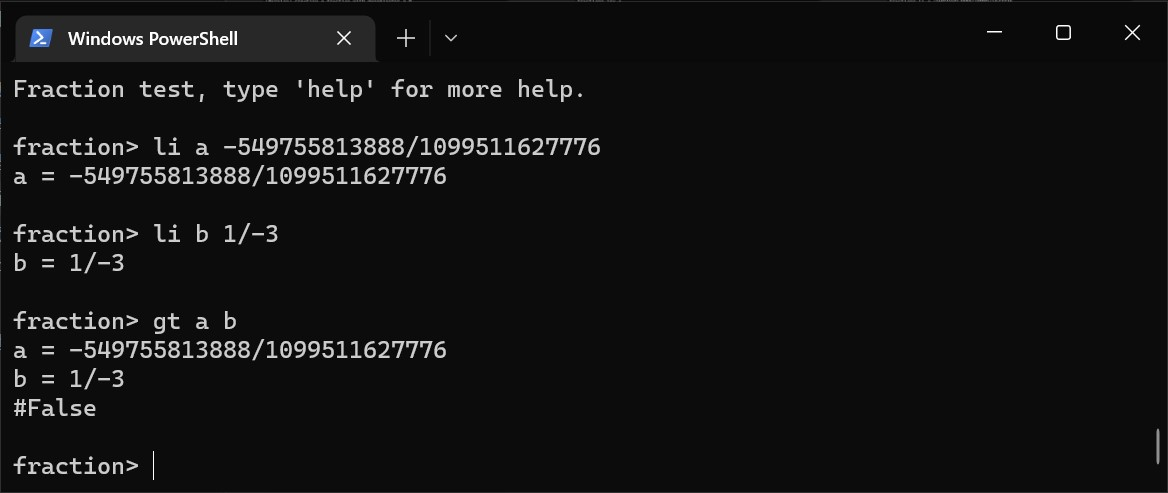
\includegraphics[width=.8\textwidth]{imgs/test_r_gt.jpg}
    \caption{比较运算-除法测试结果(符合预期)}
\end{figure}

\paragraph{小于} 测试用例 \lstinline{-549755813888/1099511627776 < 1/-3}
\begin{figure}[H]
    \centering
    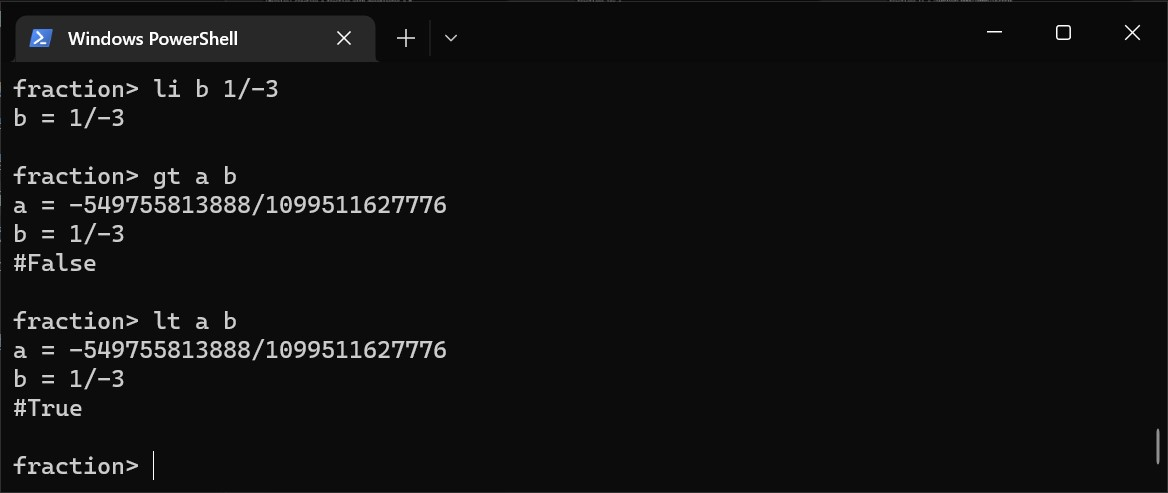
\includegraphics[width=.8\textwidth]{imgs/test_r_lt.jpg}
    \caption{比较运算-除法测试结果(符合预期)}
\end{figure}

\paragraph{等于} 测试用例 \lstinline{-549755813888/1099511627776 == 1/-3}
\begin{figure}[H]
    \centering
    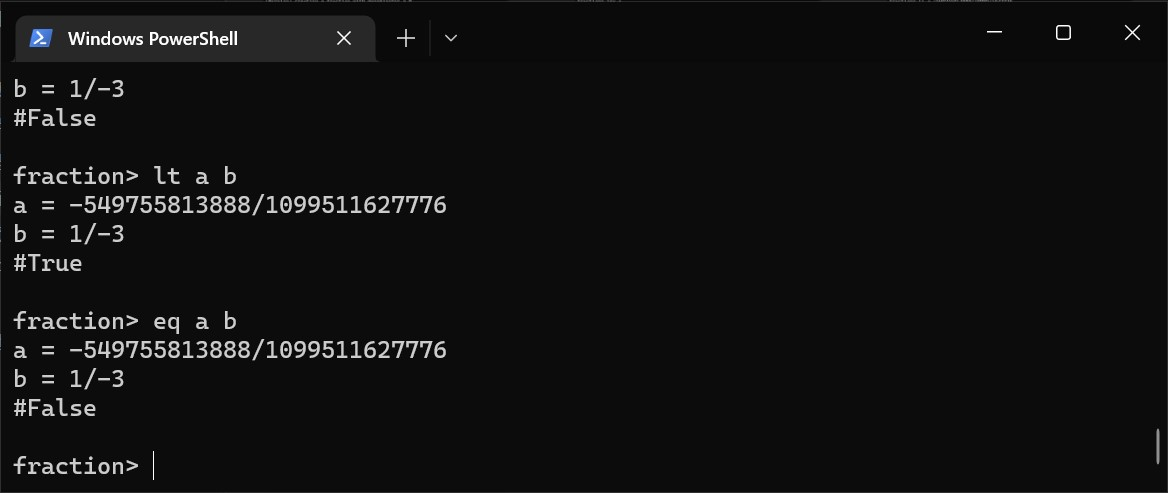
\includegraphics[width=.8\textwidth]{imgs/test_r_eq.jpg}
    \caption{比较运算-除法测试结果(符合预期)}
\end{figure}

\paragraph{大于等于} 测试用例 \lstinline{-549755813888/1099511627776 >= 1/-3}
\begin{figure}[H]
    \centering
    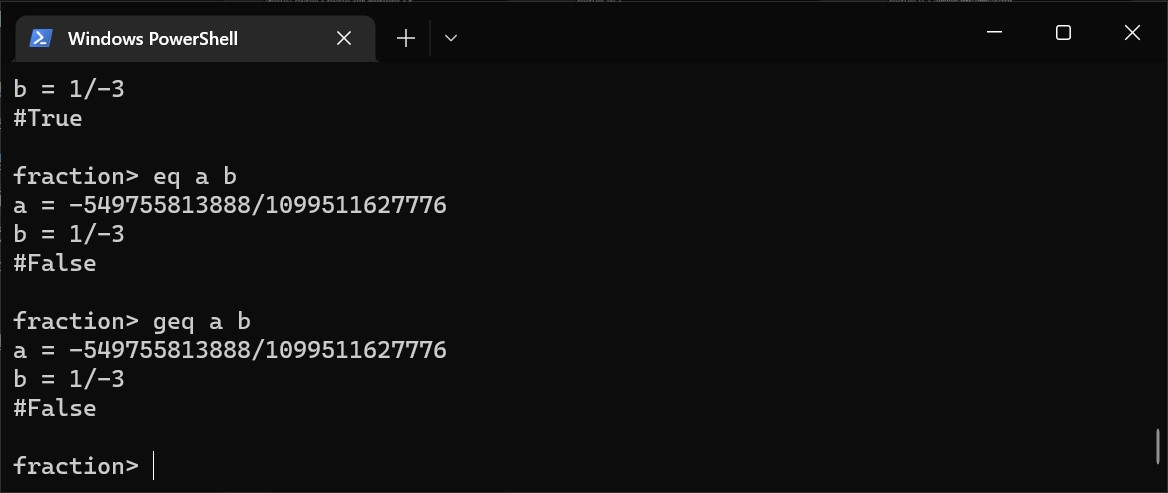
\includegraphics[width=.8\textwidth]{imgs/test_r_geq.jpg}
    \caption{比较运算-大于等于测试结果(符合预期)}
\end{figure}

\paragraph{小于等于} 测试用例 \lstinline{-549755813888/1099511627776 <= 1/-3}
\begin{figure}[H]
    \centering
    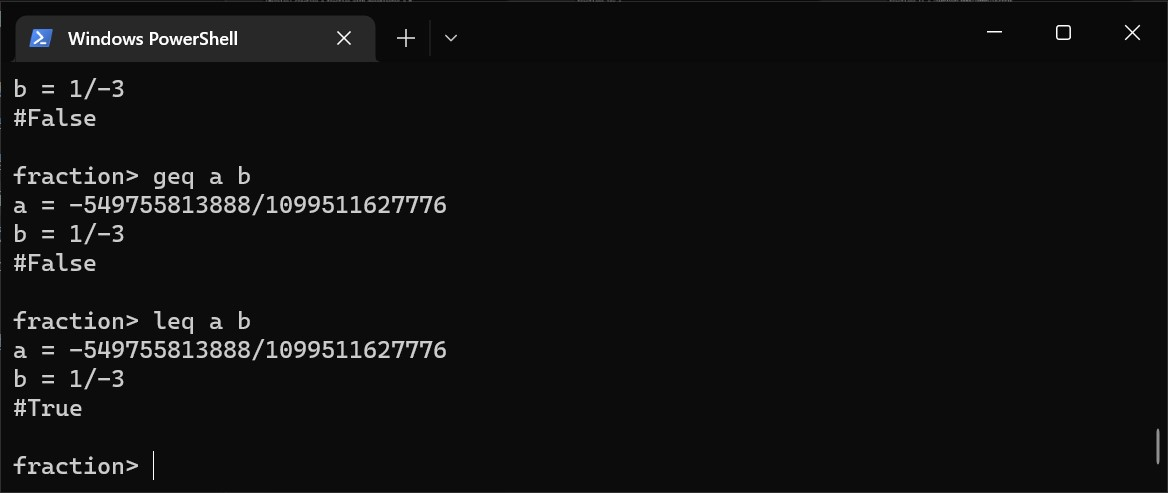
\includegraphics[width=.8\textwidth]{imgs/test_r_leq.jpg}
    \caption{比较运算-小于等于测试结果(符合预期)}
\end{figure}

\paragraph{不等于} 测试用例 \lstinline{-549755813888/1099511627776 != 1/-3}
\begin{figure}[H]
    \centering
    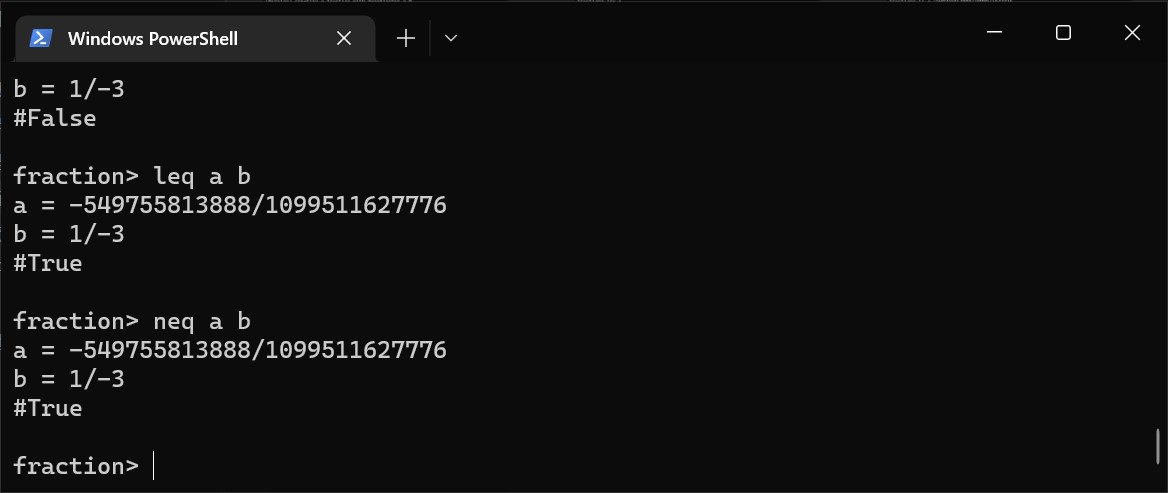
\includegraphics[width=.8\textwidth]{imgs/test_r_neq.jpg}
    \caption{比较运算-不等于测试结果(符合预期)}
\end{figure}

\section{设计思路}

\subsection{分层开发}

为了实现一个支持任意精度运算分数类,直接使用 \lstinline{int64} 等常规的数据类型是不够的。同时为了方便开发与调试,应当优先完成分数类的核心功能,即完成分数的构造,运算和比较功能的实现,然后再对其底层依赖的整数进行高精度的改造。

于是笔者使用了如下的策略:首先创建一个 \lstinline{myint} 类,该类最初是 \lstinline{int} 的简单封装,提供了整数的构造,运算和比较功能。然后,在构建 \lstinline{fraction} 类时,分子和分母使用 \lstinline{myint} 类的对象。在基于 \lstinline{myint} 类提供的接口实现并测试好 \lstinline{fraction} 类后,便着手将 \lstinline{myint} 类重构为支持高精度的版本。

重构 \lstinline{myint} 类时,为了方便调试,笔者创建了一个 \lstinline{mynat} 类用于进行高精度的自然数操作,然后在 \lstinline{myint} 中引入\lstinline{mynat} 对象和正负号,就可以方便地实现 \lstinline{fraction} 类所需要的方法。

\subsection{组合优于继承}

面向对象编程中,有一条非常经典的设计原则,那就是:组合优于继承,多用组合少用继承。这个表述最早出现在 GoF 的《Design Patterns: Elements of Reusable Object-Oriented Software》中。在本次作业中,笔者并没有让整数类继承自然数类,也没有让分数类继承整数类,而是使用组合的方式,在整数类中使用自然数类的对象并在分数类中使用整数类的对象。

这样使用组合的方式,相比使用继承的机制,有诸多优势。除了可以避免继承带来的代码重复率高的问题外,组合对象的方式对于小型项目可以方便重构的进行。一般而言,继承应当在接口和实例之间使用,而非用于实例之间。

\subsection{类图}

\begin{figure}[H]
    \centering
    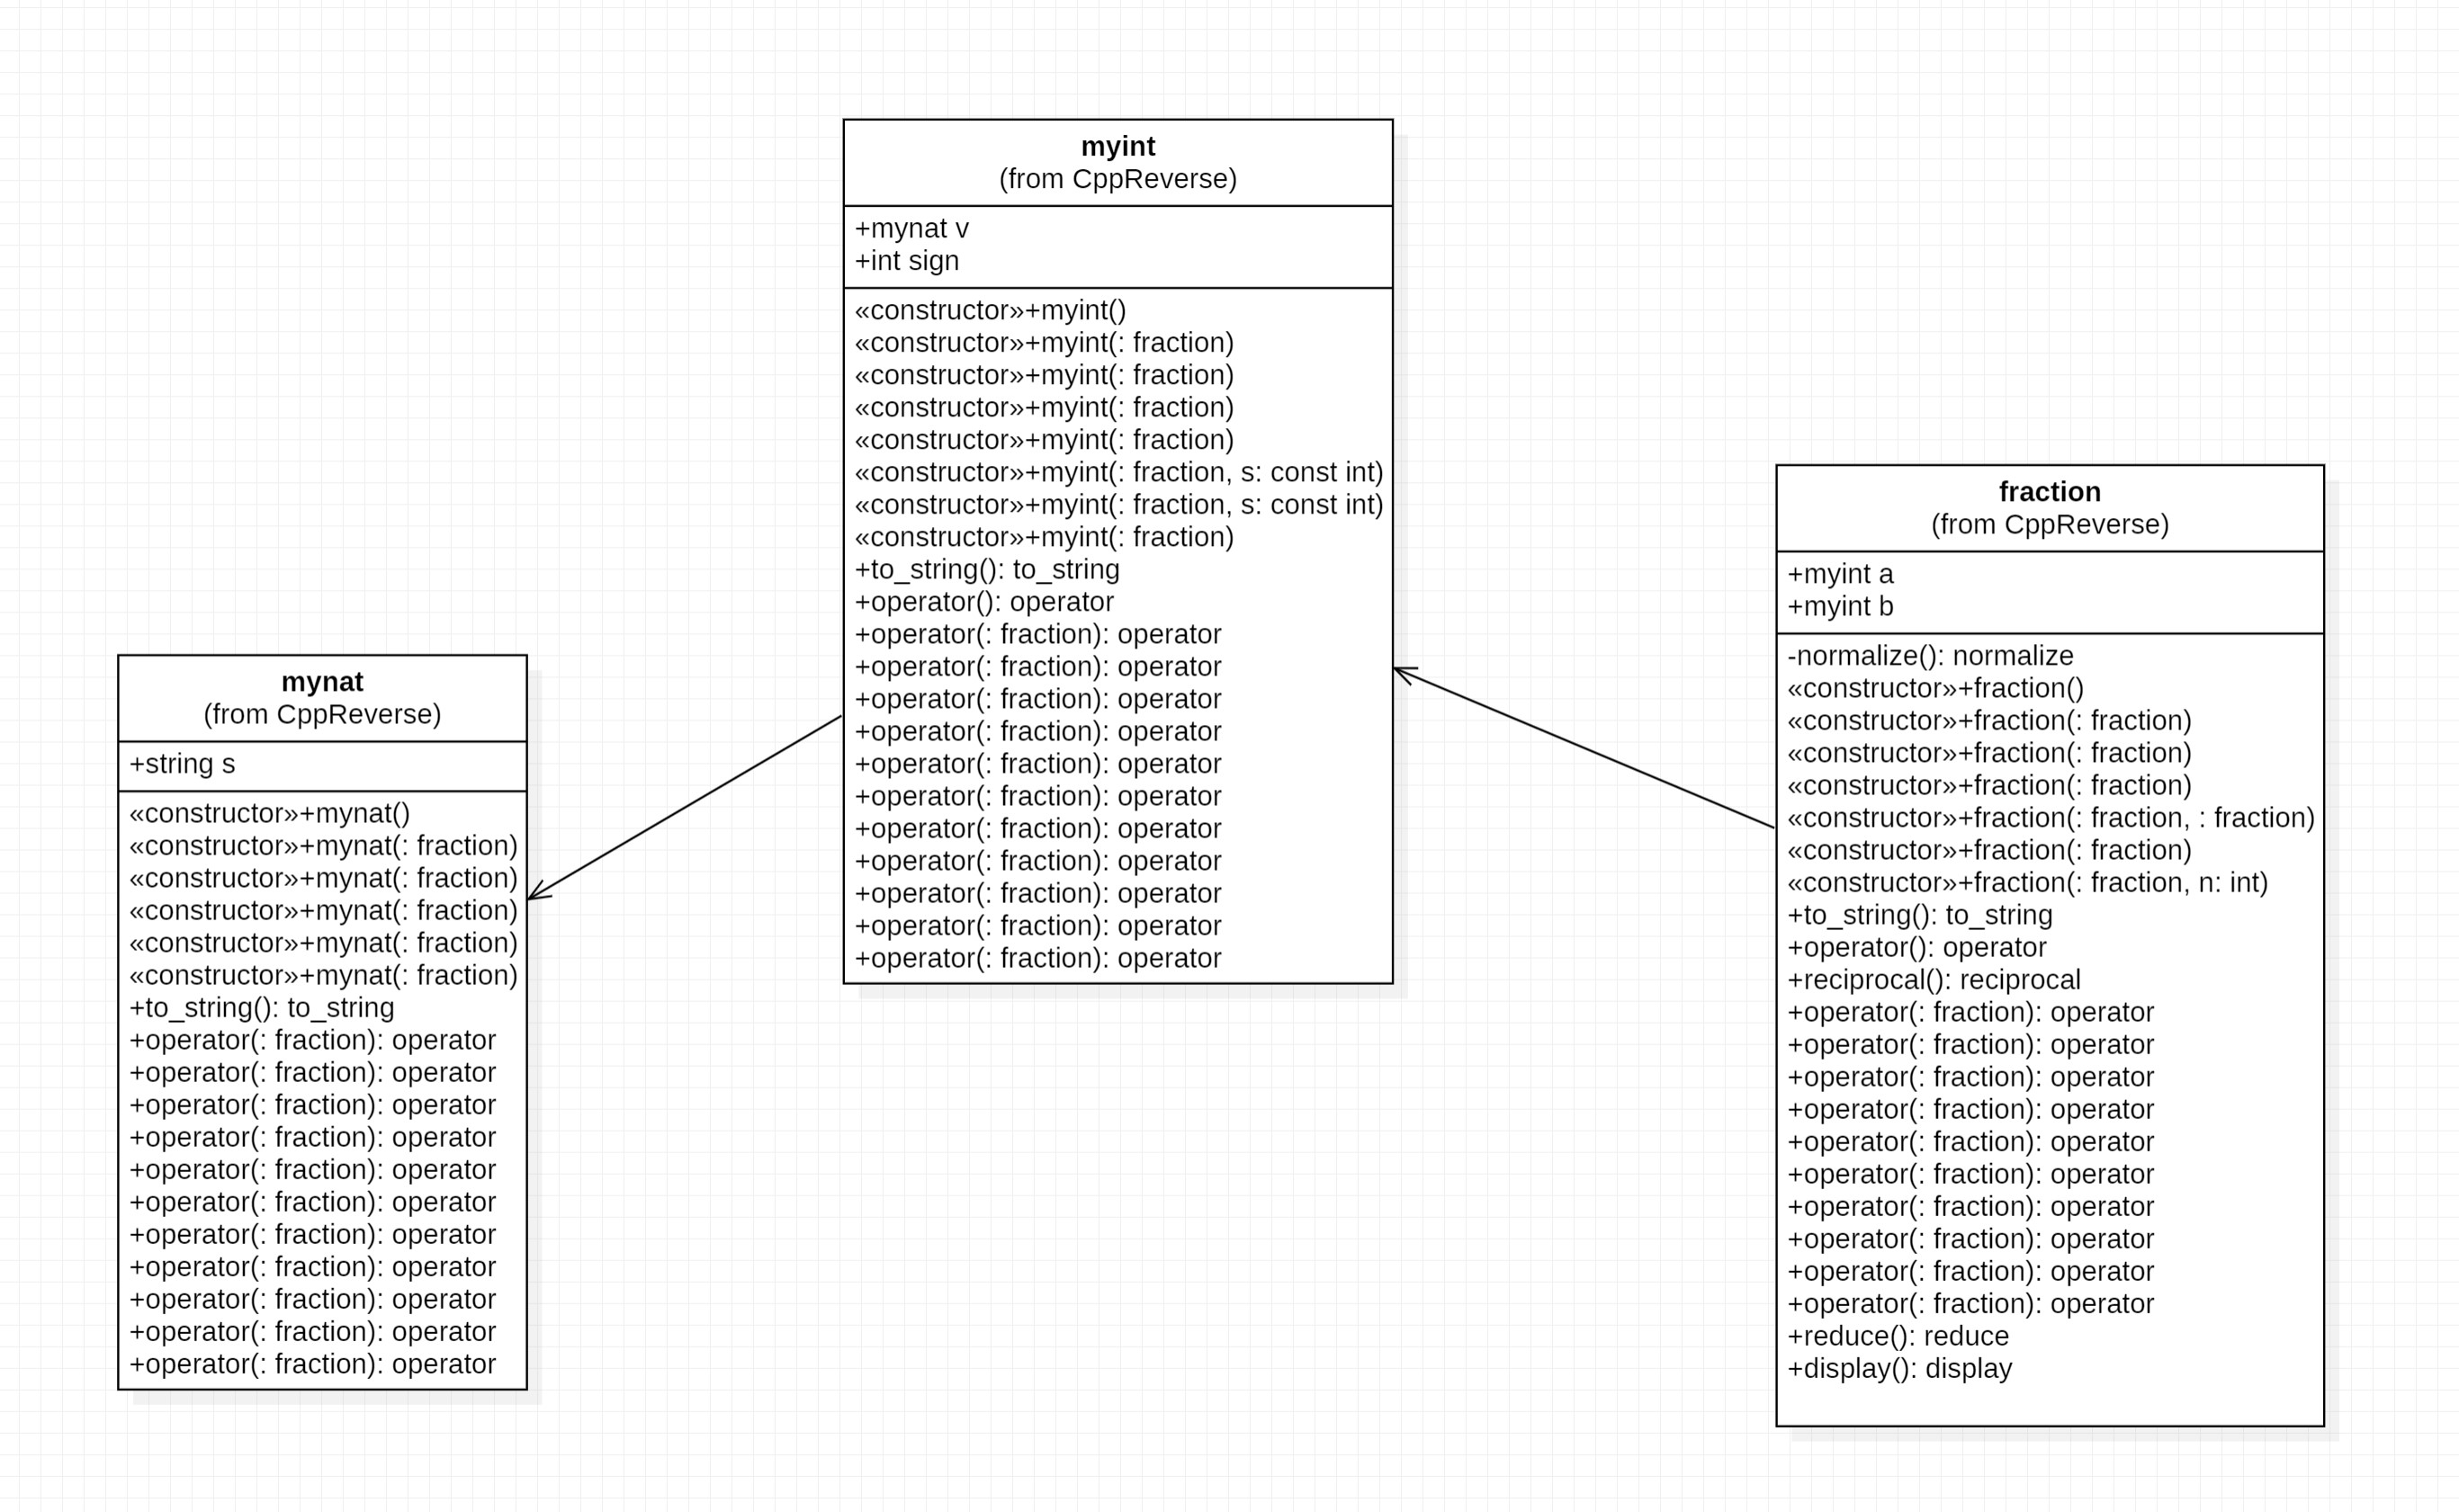
\includegraphics[width=.8\textwidth]{imgs/class_diagram.jpg}
    \caption{本次作业的类图}
\end{figure}

\section{实现细节}

\subsection{高精度正整数类}

高精度正整数类的实践主要依托 \lstinline{std::string} 类,其各个运算的实现均和正常人使用竖式进行计算的过程一致。在二次开发中值得注意的是,由于正整数不包含负数,故而重载的运算符减号实现的是两数字的差的绝对值。

在实现的细节上,\lstinline{std::string} 类用于倒序存储一个十进制整数的各位数字,即最低位存储在 \lstinline{s[0]} 中,十位存储在 \lstinline{s[1]} 中,且笔者的实现保证除了 0 以外,其余正整数的字符串中没有前导的 0 。

\subsection{高精度整数类}
高精度整数类使用一个高精度正整数类对象表示其绝对值,使用一个整数表示其符号,该整数的取值为 1 或 -1 。对于整数 0 ,我们规定其符号为正。

其余函数的实现几乎都是按操作数的符号分情况讨论,并直接调用正整数类的成员函数。二次开发时,注意取操作结果的正负号只与被取模的数一致。

\subsection{高精度分数类}
高精度分数类使用两个正整数类对象分别表示分子和分母,一个高精度分数类对象的标准形式为:分子符号表示分数的符号,分母的符号为正,且分子分母的最大公因数为 1 。

高精度分数类对象的四则运算主要基于正常的通分进行,且结果不会进行标准化,因为按照作业的要求,对于一个分数的约分和标准化是需要手动进行的。在出现分母为 0 的情况时,分数类会报异常,并且此时的计算结果是不可信的。

\section{作业小结}

在本次作业中,笔者完成了 \lstinline{fraction} 类的构建与测试,从而实践了面向对象程序设计中的一些基本概念,例如封装和多态等。作业中通过构造自然数类和整数类,从而完成了分数类的构建,从而实践了面向对象程序设计的一些思路。

笔者构建的分数类的计算效率主要取决于自然数类的实现,如果将自然数类中的乘法使用 FFT (快速傅里叶变换)或者 NTT (快速数论变换)进行改进,则可以较大地提升性能,而无需修改整数类或者分数类的实现。

\end{document}